\documentclass{beamer}
\usepackage{amsmath,amssymb}
\usepackage{tikz}
\usepackage{enumerate}
\usepackage{xcolor}
\usepackage{algorithm2e}

% Theorems
\usepackage{amsthm}
\renewcommand\qedsymbol{$\blacksquare$}
\makeatletter
\@ifclassloaded{article}{
    \newtheorem{definition}{Definition}[section]
    \newtheorem{example}{Example}[section]
    \newtheorem{theorem}{Theorem}[section]
    \newtheorem{corollary}{Corollary}[theorem]
    \newtheorem{lemma}{Lemma}[theorem]
}{
}
\makeatother

% Random Stuff
\setlength\unitlength{1mm}

\newcommand{\insertfig}[3]{
\begin{figure}[htbp]\begin{center}\begin{picture}(120,90)
\put(0,-5){\includegraphics[width=12cm,height=9cm,clip=]{#1.eps}}\end{picture}\end{center}
\caption{#2}\label{#3}\end{figure}}

\newcommand{\insertxfig}[4]{
\begin{figure}[htbp]
\begin{center}
\leavevmode \centerline{\resizebox{#4\textwidth}{!}{\input
#1.pstex_t}}
\caption{#2} \label{#3}
\end{center}
\end{figure}}

\long\def\comment#1{}

\newcommand\norm[1]{\left\lVert#1\right\rVert}
\DeclareMathOperator*{\argmin}{arg\,min}
\DeclareMathOperator*{\argmax}{arg\,max}

% bb font symbols
\newfont{\bbb}{msbm10 scaled 700}
\newcommand{\CCC}{\mbox{\bbb C}}

\newfont{\bbf}{msbm10 scaled 1100}
\newcommand{\CC}{\mbox{\bbf C}}
\newcommand{\PP}{\mbox{\bbf P}}
\newcommand{\RR}{\mbox{\bbf R}}
\newcommand{\QQ}{\mbox{\bbf Q}}
\newcommand{\ZZ}{\mbox{\bbf Z}}
\renewcommand{\SS}{\mbox{\bbf S}}
\newcommand{\FF}{\mbox{\bbf F}}
\newcommand{\GG}{\mbox{\bbf G}}
\newcommand{\EE}{\mbox{\bbf E}}
\newcommand{\NN}{\mbox{\bbf N}}
\newcommand{\KK}{\mbox{\bbf K}}
\newcommand{\KL}{\mbox{\bbf KL}}

% Vectors
\renewcommand{\aa}{{\bf a}}
\newcommand{\bb}{{\bf b}}
\newcommand{\cc}{{\bf c}}
\newcommand{\dd}{{\bf d}}
\newcommand{\ee}{{\bf e}}
\newcommand{\ff}{{\bf f}}
\renewcommand{\gg}{{\bf g}}
\newcommand{\hh}{{\bf h}}
\newcommand{\ii}{{\bf i}}
\newcommand{\jj}{{\bf j}}
\newcommand{\kk}{{\bf k}}
\renewcommand{\ll}{{\bf l}}
\newcommand{\mm}{{\bf m}}
\newcommand{\nn}{{\bf n}}
\newcommand{\oo}{{\bf o}}
\newcommand{\pp}{{\bf p}}
\newcommand{\qq}{{\bf q}}
\newcommand{\rr}{{\bf r}}
\renewcommand{\ss}{{\bf s}}
\renewcommand{\tt}{{\bf t}}
\newcommand{\uu}{{\bf u}}
\newcommand{\ww}{{\bf w}}
\newcommand{\vv}{{\bf v}}
\newcommand{\xx}{{\bf x}}
\newcommand{\yy}{{\bf y}}
\newcommand{\zz}{{\bf z}}
\newcommand{\0}{{\bf 0}}
\newcommand{\1}{{\bf 1}}

% Matrices
\newcommand{\Ab}{{\bf A}}
\newcommand{\Bb}{{\bf B}}
\newcommand{\Cb}{{\bf C}}
\newcommand{\Db}{{\bf D}}
\newcommand{\Eb}{{\bf E}}
\newcommand{\Fb}{{\bf F}}
\newcommand{\Gb}{{\bf G}}
\newcommand{\Hb}{{\bf H}}
\newcommand{\Ib}{{\bf I}}
\newcommand{\Jb}{{\bf J}}
\newcommand{\Kb}{{\bf K}}
\newcommand{\Lb}{{\bf L}}
\newcommand{\Mb}{{\bf M}}
\newcommand{\Nb}{{\bf N}}
\newcommand{\Ob}{{\bf O}}
\newcommand{\Pb}{{\bf P}}
\newcommand{\Qb}{{\bf Q}}
\newcommand{\Rb}{{\bf R}}
\newcommand{\Sb}{{\bf S}}
\newcommand{\Tb}{{\bf T}}
\newcommand{\Ub}{{\bf U}}
\newcommand{\Wb}{{\bf W}}
\newcommand{\Vb}{{\bf V}}
\newcommand{\Xb}{{\bf X}}
\newcommand{\Yb}{{\bf Y}}
\newcommand{\Zb}{{\bf Z}}

% Calligraphic
\newcommand{\Ac}{{\cal A}}
\newcommand{\Bc}{{\cal B}}
\newcommand{\Cc}{{\cal C}}
\newcommand{\Dc}{{\cal D}}
\newcommand{\Ec}{{\cal E}}
\newcommand{\Fc}{{\cal F}}
\newcommand{\Gc}{{\cal G}}
\newcommand{\Hc}{{\cal H}}
\newcommand{\Ic}{{\cal I}}
\newcommand{\Jc}{{\cal J}}
\newcommand{\Kc}{{\cal K}}
\newcommand{\Lc}{{\cal L}}
\newcommand{\Mc}{{\cal M}}
\newcommand{\Nc}{{\cal N}}
\newcommand{\Oc}{{\cal O}}
\newcommand{\Pc}{{\cal P}}
\newcommand{\Qc}{{\cal Q}}
\newcommand{\Rc}{{\cal R}}
\newcommand{\Sc}{{\cal S}}
\newcommand{\Tc}{{\cal T}}
\newcommand{\Uc}{{\cal U}}
\newcommand{\Wc}{{\cal W}}
\newcommand{\Vc}{{\cal V}}
\newcommand{\Xc}{{\cal X}}
\newcommand{\Yc}{{\cal Y}}
\newcommand{\Zc}{{\cal Z}}

% Bold greek letters
\newcommand{\alphab}{\hbox{\boldmath$\alpha$}}
\newcommand{\betab}{\hbox{\boldmath$\beta$}}
\newcommand{\gammab}{\hbox{\boldmath$\gamma$}}
\newcommand{\deltab}{\hbox{\boldmath$\delta$}}
\newcommand{\etab}{\hbox{\boldmath$\eta$}}
\newcommand{\lambdab}{\hbox{\boldmath$\lambda$}}
\newcommand{\epsilonb}{\hbox{\boldmath$\epsilon$}}
\newcommand{\nub}{\hbox{\boldmath$\nu$}}
\newcommand{\mub}{\hbox{\boldmath$\mu$}}
\newcommand{\zetab}{\hbox{\boldmath$\zeta$}}
\newcommand{\phib}{\hbox{\boldmath$\phi$}}
\newcommand{\psib}{\hbox{\boldmath$\psi$}}
\newcommand{\thetab}{\hbox{\boldmath$\theta$}}
\newcommand{\taub}{\hbox{\boldmath$\tau$}}
\newcommand{\omegab}{\hbox{\boldmath$\omega$}}
\newcommand{\xib}{\hbox{\boldmath$\xi$}}
\newcommand{\sigmab}{\hbox{\boldmath$\sigma$}}
\newcommand{\pib}{\hbox{\boldmath$\pi$}}
\newcommand{\rhob}{\hbox{\boldmath$\rho$}}

\newcommand{\Gammab}{\hbox{\boldmath$\Gamma$}}
\newcommand{\Lambdab}{\hbox{\boldmath$\Lambda$}}
\newcommand{\Deltab}{\hbox{\boldmath$\Delta$}}
\newcommand{\Sigmab}{\hbox{\boldmath$\Sigma$}}
\newcommand{\Phib}{\hbox{\boldmath$\Phi$}}
\newcommand{\Pib}{\hbox{\boldmath$\Pi$}}
\newcommand{\Psib}{\hbox{\boldmath$\Psi$}}
\newcommand{\Thetab}{\hbox{\boldmath$\Theta$}}
\newcommand{\Omegab}{\hbox{\boldmath$\Omega$}}
\newcommand{\Xib}{\hbox{\boldmath$\Xi$}}

% mixed symbols
\newcommand{\sinc}{{\hbox{sinc}}}
\newcommand{\diag}{{\hbox{diag}}}
\renewcommand{\det}{{\hbox{det}}}
\newcommand{\trace}{{\hbox{tr}}}
\newcommand{\tr}{\trace}
\newcommand{\sign}{{\hbox{sign}}}
\renewcommand{\arg}{{\hbox{arg}}}
\newcommand{\var}{{\hbox{var}}}
\newcommand{\cov}{{\hbox{cov}}}
\renewcommand{\Re}{{\rm Re}}
\renewcommand{\Im}{{\rm Im}}
\newcommand{\eqdef}{\stackrel{\Delta}{=}}
\newcommand{\defines}{{\,\,\stackrel{\scriptscriptstyle \bigtriangleup}{=}\,\,}}
\newcommand{\<}{\left\langle}
\renewcommand{\>}{\right\rangle}
\newcommand{\Psf}{{\sf P}}
\newcommand{\T}{\top}
\newcommand{\m}[1]{\begin{bmatrix} #1 \end{bmatrix}}

\beamertemplatenavigationsymbolsempty

\title{A Brisk Overview of Convex Optimization}
\subtitle{Looking at Figures That Took Too Long to Make.}
\author{Conner DiPaolo}
\institute{Harvey Mudd College / Yelp}
\date{August, 2016}

\AtBeginSection[]
{
    \begin{frame}
        \frametitle{Table of Contents}
        \tableofcontents[currentsection]
    \end{frame}
}

\begin{document}

\frame{\titlepage}

\section{Overview}
\begin{frame}
    \frametitle{Convex Optimization}
    \begin{enumerate}
        \item Core behind techniques in machine learning, signal processing, operations research, etc.
        \item Can be \textit{very} applied or very theoretical
        \item If you need more resources check out \textit{Convex Optimization} by Boyd and
            Vandenberghe\footnote{\url{http://stanford.edu/~boyd/cvxbook/}}.
    \end{enumerate}
\end{frame}

\section{Set Convexity}
\begin{frame}
    \frametitle{Convex Sets}
    \begin{center}
        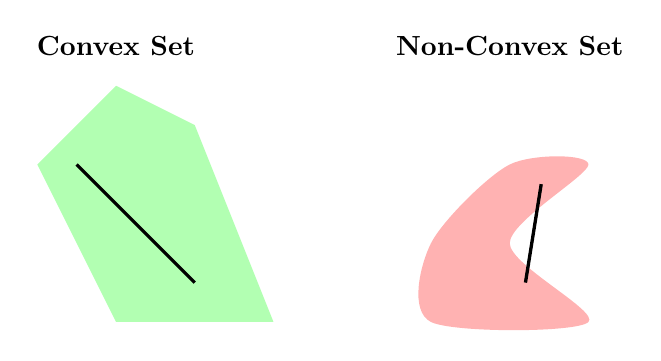
\begin{tikzpicture}
            \begin{scope}[shift={(-2,0)}]
                \draw (0,3.5) node {\textbf{Convex Set}};
                \fill[color=green!30] (0,0) -- (-1,2) -- (0,3) -- (1,2.5) -- (2,0)  -- cycle;
                \draw[very thick] (-0.5,2) -- (1,0.5);
            \end{scope}
            \begin{scope}[shift={(2,0)}]
                \draw (1,3.5) node {\textbf{Non-Convex Set}};
                \fill[color=red!30] plot [smooth cycle] coordinates {(0,1) (1,2) (2,2) (1,1) (2,0) (0,0)};
                \draw[very thick] (1.4,1.75) -- (1.2,0.5);
            \end{scope}
        \end{tikzpicture}
    \end{center}
\end{frame}

\begin{frame}
    \frametitle{Convex Sets - an Intuitive Definition}
    A set $C$ is \textit{convex} if, given any two points in that set, every point on the line
    segment between those two points is also in $C$.
\end{frame}

\begin{frame}
    \frametitle{Convex Sets}
    \begin{definition}[Convex Combination / Line Segment]
        A convex combination of two points $\xx$ and $\yy$ from an affine space is
        \[
            \theta\xx + (1-\theta)\yy,
        \]
        where $0\leq\theta\leq1$.\\[2em]
    \end{definition}

    \begin{center}
        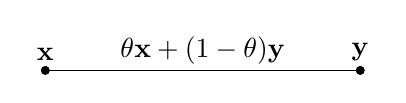
\begin{tikzpicture}
            \draw[fill=black] (0,0) circle (0.05) node[above] {$\xx$};
            \draw[fill=black] (4,0) circle (0.05) node[above] {$\yy$};
            \draw (0,0) -- (4,0);
            \draw (2,0.25) node {$\theta\xx + (1-\theta)\yy$};
        \end{tikzpicture}
    \end{center}
\end{frame}

\begin{frame}
    \frametitle{Convex Sets - an Actual Definition}
    A set $C$ is \textit{convex} if, given any two points in that set, every point on the line
    segment between those two points is also in $C$. Mathematically, we have

    \begin{definition}[Convex Set]
        A set $C$ is convex if, given $\xx, \yy\in C$, every convex combination of $\xx$ and $\yy$
        still lies in $C$. That is,
        \[
            \theta\xx + (1-\theta)\yy \in C. \tag{$0\leq\theta\leq1$}
        \]
        for all $\xx$ and $\yy$ in $C$.
    \end{definition}
\end{frame}

\begin{frame}
    \frametitle{Convex Sets}
    \begin{example}[The Space of Probability Distributions]
        Let $\Pc$ be the space of continuous probability distributions over
        $\RR^n$. That is, every element of $\Pc$ defines a unique probability
        density function $\PP(x) \geq 0$ such that \[\int_{\RR^n} \PP(x) dx=1.\]
        $\Pc$ is convex.
    \end{example}
\end{frame}

\begin{frame}
    \frametitle{Convex Sets}
    \begin{proof}
        Let $f$ and $h$ be valid probability distributions from $\Pc$. That is,
        \[
            f,h \in \left\{\PP(x) : \int_{\RR^n} \PP(x)dx = 1 \text{ and } \PP(x) \geq 0 \right\}.
        \]
        Now let $0\leq\theta\leq1$. Then
        \[
            \theta f(x) + (1-\theta) h(x) \geq 0
        \]
        as a positive combination of positive functions. Similarly,
        \begin{align*}
            \int_{\RR^n}\left[ \theta f(x) + (1-\theta) h(x) \right]dx &= \theta\int_{\RR^n}f(x)dx + (1-\theta)\int_{\RR^n}h(x)dx\\
            &= \theta + (1-\theta) = 1.
        \end{align*}
    \end{proof}
\end{frame}

\section{Function Convexity}

\begin{frame}
    \frametitle{Convex Functions}
    \begin{center}
        \begin{tikzpicture}
            \begin{scope}[shift={(-3.75,0)},scale=0.75]
                \draw[domain=-1.75:1.75,
                      smooth,
                      variable=\x,
                      blue] plot ({\x},{\x*\x/4});
                \draw (0, 4) node {\textbf{Convex Function}};
            \end{scope}
            \begin{scope}[shift={(0,0)},scale=0.75]
                \draw[domain=-1.75:1.75,
                      smooth,
                      variable=\x,
                      blue] plot ({\x},{-\x*\x/4 + 1});
                \draw (0, 4) node {\textbf{Concave Function}};
            \end{scope}
            \begin{scope}[shift={(3.75,0)},scale=0.75]
                \draw[domain=-1.75:1.75,
                      smooth,
                      variable=\x,
                      blue] plot ({\x},{\x*\x*\x/4 + 0.5});
                \draw (0, 4) node {\textbf{Neither}};
            \end{scope}
        \end{tikzpicture}
    \end{center}
\end{frame}

\begin{frame}
    \frametitle{Convex Function}
    \begin{definition}[Convex Function]
    A function $f : C \mapsto \RR$ is \textit{convex} if its domain $C$ is convex and,
    for $0\leq\theta\leq1$, given any $\xx, \yy\in C$,
    \[
        f(\theta\xx + (1-\theta)\yy) \leq \theta f(\xx) + (1-\theta)f(\yy).
    \]
    That is, a line segment drawn between two function values lies above the function.
    \end{definition}
\end{frame}

\begin{frame}
    \frametitle{Convex Function}
    \begin{center}
        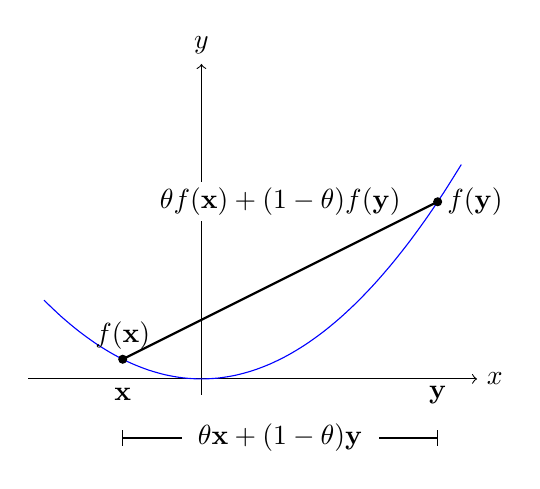
\begin{tikzpicture}
            \begin{scope}[shift={(-3,0)}]
                \draw[->] (-2.2,0) -- (3.5,0) node[right] {$x$};
                \draw[->] (0,-0.2) -- (0,4) node[above] {$y$};
                \draw[domain=-2:3.3,
                      smooth,
                      variable=\x,
                      blue] plot ({\x},{\x*\x/4});
                \fill[color=white] (-1,2) rectangle (2.75,2.5);
                \draw[fill=black] (-1,0.25) circle (0.05) node[above]{$f(\xx)$};
                \draw[fill=black] (3,2.25) circle (0.05) node[right]{$f(\yy)$};
                \draw (-1,-0.2) node {$\xx$};
                \draw (3,-0.2) node {$\yy$};
                \draw[thick] (-1,0.25) -- (3,2.25);
                \draw (1,2.25) node {$\theta f(\xx) + (1-\theta)f(\yy)$};
                \draw (1,-0.75) node {$\theta \xx + (1-\theta)\yy$};
                \draw (-1,-0.75) -- ++(0,0.1) -- ++(0,-0.2) -- ++(0,0.1) -- ++(0.75,0);
                \draw (3,-0.75) -- ++(0,0.1) -- ++(0,-0.2) -- ++(0,0.1) -- ++(-0.75,0);
            \end{scope}

            \begin{scope}[shift={(-3,0)}]
            \end{scope}
        \end{tikzpicture}
    \end{center}
\end{frame}

\begin{frame}
    \frametitle{Second Order Conditions}
    \begin{theorem}
        A twice differentiable function $f : \RR^n \mapsto \RR$ is convex if and only if
        it's Hessian is positive semi-definite:
        \[
            \nabla^2 f \succeq 0.
        \]
    \end{theorem}
\end{frame}

\begin{frame}
    \frametitle{Concave and Convex Functions}
    \begin{example}
        $f(x) = \log(x) : \RR_{++} \mapsto \RR$ is concave.
    \end{example}
    \begin{proof}
        $f''(x) = -\frac{1}{x^2} < 0$, so $f$ is \textit{strictly concave}.
    \end{proof}
    \begin{example}
        $f(x) = \exp(x) : \RR \mapsto \RR_{++}$ is convex.
    \end{example}
    \begin{proof}
        $f''(x) = e^x > 0$, so $f$ is \textit{strictly convex}.
    \end{proof}
\end{frame}

\begin{frame}
    \frametitle{Convex Function}
    \begin{example}
        The function $f : \RR^n \mapsto \RR$ defined by
        \[
            f(\xx) = e^{\xx^\T\xx} = e^{\xx_1^2 + \dots + \xx_n^2}
        \]
        is convex.
    \end{example}
    \begin{proof}
        Each element of the Hessian
        \begin{align*}
            \nabla^2f_{ij} &= \frac{\partial^2 f}{\partial x_i \partial x_j} = 4\xx_i\xx_j e^{\xx^\T\xx}\\
            \nabla^2f &= 4\xx\xx^\T e^{\xx^\T\xx}.
        \end{align*}
        Is this positive semi-definite? Consider $\zz\in\RR^n$. Then
        \[
            \zz^\T\nabla^2 f(x)\zz = \zz^\T4\xx\xx^\T e^{\xx^\T\xx} \zz = 4(\zz^\T\xx)^2 e^{\xx^\T\xx} \geq 0
        \]
    \end{proof}
\end{frame}

\begin{frame}
    \frametitle{Convex Function}
    \begin{example}[Quadratic Functions]
        The function $f : \RR^n \mapsto \RR$ defined by
        \[
            f(\xx) = \xx^\T A\xx + \bb^\T\xx + c
        \]
        is convex if $A \succeq 0$.
    \end{example}
    \begin{proof}
        We know
        \[
            \nabla^2 f = 2A.
        \]
        Similarly we know that $2A \succeq 0$ if and only if
        $A \succeq 0$. Thus by the second order conditions $f$
        is convex if and only if $A \succeq 0$.\\

        We can also show that $f$ is concave if $A\preceq 0$.
    \end{proof}
\end{frame}

\begin{frame}
    \frametitle{Affine Composition}
    \begin{theorem}
        Given a convex $f : \RR^m \mapsto \RR$, any matrix $A\in\RR^{m \times n}$, $\xx\in\RR^n$,
        and $\bb\in\RR^m$,
        \[
            g(\xx) = f(A\xx + \bb)
        \]
        is convex.
    \end{theorem}
    \begin{proof}
        \[
            \nabla^2g = A^\T \nabla^2 f(A\xx + \bb) A.
        \]
        Then, for any $\zz\in\RR^n$,
        \[
            \zz^\T \nabla^2g \zz = \zz^\T A^\T \nabla^2 f(A\xx + \bb) A \zz = (A\zz)^\T\nabla^2 f(A\xx + \bb) (A \zz) \geq 0
        \]
        by the convexity assumption, so $g$ is convex.
    \end{proof}
\end{frame}

\section{(Convex and Not) Optimization Problems}
\begin{frame}
    \frametitle{Optimization Problems}
    An optimization problem is a problem of the form
    \begin{align*}
        \text{minimize: } & f_0(\xx)\\
        \text{subj. to: } & f_i(\xx) \leq 0, \quad i=1,\dots,m\\
                          & h_i(\xx) = 0, \quad i=1,\dots,p
    \end{align*}
    The goal of an optimization problem, as you might be able to guess, is to optimize $f_0$
    where $\xx$ is in the problem domain domain 
    \[
        \Dc = \bigcap_{i=0}^m\mathbf{dom}\; f_i \;\cap\; \bigcap_{i=1}^p \mathbf{dom}\; h_i,
    \]
    satisfying the problem constraints.
\end{frame}

\begin{frame}
    \frametitle{Convex Optimization Problems}
    An optimization problem of the form
    \begin{align*}
        \text{minimize: } & f_0(\xx)\\
        \text{subj. to: } & f_i(\xx) \leq 0, \quad i=1,\dots,m\\
                          & A\xx = \bb
    \end{align*}
    is convex if $f_i$ for all $i = 0,\dots,m$ are convex.
\end{frame}

\begin{frame}
    \frametitle{Global Optimality of Convex Optimization Problems}
    
    \begin{theorem}[Global Optimality]
        Given a convex optimization problem, and local optimum $\xx^\star$
        such that
        \[
            f_0(\xx) = \inf\{f_0(\zz) : \zz\text{ feasible and } ||\zz-\xx||_2 \leq R\}
        \]
        for some $R > 0$. $\xx^\star$ is the global optimum.
    \end{theorem}
    \begin{proof}
        (Boyd)
        Suppose local optimality but not global optimality, with some feasible $\yy$
        such that $f_0(\yy) < f_0(\xx)$. Then $||\yy-\xx||_2 >R$ because otherwise $f_0(\xx)
        \leq f_0(\yy)$. Consider a point $\zz$ given by
        \[
            \zz = (1-\theta)\xx+ \theta\yy \quad\text{and}\quad \theta=\frac{R}{2||\yy-\xx||_2}.
        \]
        Then $||\xx-\zz||_2=R/2 < R$. By convexity of the feasible set,
        $\zz$ is feasible. By the convexity of the objective function $f_0$
        we have
        \[
            f_0(\zz) \leq (1-\theta)f_0(\xx) + \theta f_0(\yy) < f_0(\xx)
        \]
    \end{proof}
\end{frame}

\begin{frame}
    \frametitle{Common Problems - Linear Programs}

    \begin{align*}
        \text{minimize: } & \cc^\T\xx\\
        \text{subj. to: } & G\xx \preceq \hh,\\
                          & A\xx = \bb
    \end{align*}
\end{frame}

\begin{frame}
    \frametitle{Common Problems - Quadratic Programs}

    \begin{align*}
        \text{minimize: } & \frac{1}{2}\xx^\T P\xx + \qq^\T\xx + \rr\\
        \text{subj. to: } & G\xx \preceq\hh\\
                          & A\xx = \bb
    \end{align*}
    with $P \in \SS_+^n$
\end{frame}

\begin{frame}
    \frametitle{Example Problem - Analytic Centering}
    Want to find some sort of `center' of a convex polygon (polytope) $A\xx \preceq \bb$:
    \begin{align*}
        \text{minimize: } f_0(\xx) = -\sum_{i}\log(\bb_i - a_i^\T\xx)
    \end{align*}

    \begin{figure}
        \centering
        \includegraphics[width=0.7\linewidth]{../fig/analytic_centering.pdf}
    \end{figure}
\end{frame}

\begin{frame}
    \frametitle{Example Problem - Least Squares Linear Regression}
    We have an overdetermined (tall $A$) system $A\xx = \bb$ we want to solve,
    and we want to find the ``best'' solution by minimizing
    \[
        f = ||A\xx - \bb||_2 = (A\xx-\bb)^\T(A\xx-\bb) = \xx^\T A^\T A\xx - 2\xx^\T A^\T\bb + \bb^\T\bb.
    \]
    At optimality $\nabla f = 0$, so we can find
    \[
        \nabla f = 2A^\T A\xx - 2A^\T\bb = \0,
    \]
    so
    \[
        \xx^\star = (A^\T A)^{-1} A^\T\bb.
    \]
\end{frame}

\begin{frame}
    \frametitle{Example Problem - Logistic Regression}
    Have a dataset $\{\xx_i, y_i\}_1^m$ with $y\in \{0,1\}$. We want to predict
    \[
        \hat y = \PP(y_i = 1 | \xx_i ; \thetab) = \sigma(\thetab^\T\xx) = \frac{1}{1 + \exp(-\thetab^\T\xx)}.
    \]
    Optimization problem: maximize the (log) likelihood of our data given the parameters
    $\thetab$:
    \begin{align*}
        \text{maximize: } \log \PP(\Dc | \thetab) &= \sum_{i=1}^m y_i\log\sigma(\thetab^\T\xx) + (1-y_i)\log(1-\sigma(\thetab^\T\xx))\\
        &= \sum_{i=1}^m \ell_i
    \end{align*}
\end{frame}

\begin{frame}
    \frametitle{Example Problem - Logistic Regression}
    Is this convex? Note $\sigma'(x) = \sigma(x)\left[1 - \sigma(x)\right]$.
    Then
    \begin{align*}
        \nabla \ell &= y\xx\frac{\sigma(\thetab^\T\xx)\left[ 1-\sigma(\thetab^\T\xx) \right]}{\sigma(\thetab^\T\xx)} - (1-y)\xx\frac{\sigma(\thetab^\T\xx)\left[ 1-\sigma(\thetab^\T\xx) \right]}{1-\sigma(\thetab^\T\xx)}\\
        &= y\xx\left[1 - \sigma(\thetab^\T\xx)\right] - (1-y)\xx\sigma(\thetab^\T\xx) = \left[y-\sigma(\thetab^T\xx)\right]\xx
    \end{align*}
    and then
    \begin{align*}
        \nabla^2 \ell &= -\sigma(\thetab^\T\xx)\left[1 - \sigma(\thetab^\T\xx)\right]\xx\xx^\T \preceq 0
    \end{align*}
\end{frame}

\section{Algorithms}
\begin{frame}
    \frametitle{Optimal Solutions}
    For convex unconstrained problems
    \[
        \text{minimize: } f_0(\xx) = f(\xx)
    \]
    The optimal solution occurs when $\nabla f = \0$.
\end{frame}

\begin{frame}
    \frametitle{Gradient Descent}
    Dumb algorithm: start somewhere and take small steps down the hill.\\[3em]

    \begin{center}
        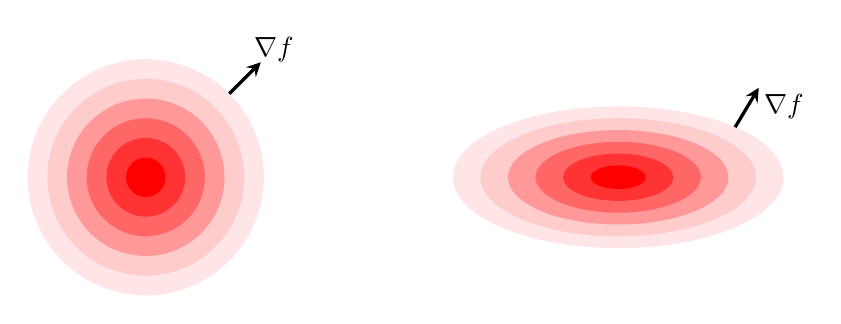
\begin{tikzpicture}
            \begin{scope}[shift={(-3,0)}]
                \fill[color=red!10] (0,0) circle (0.25*6);
                \fill[color=red!20] (0,0) circle (0.25*5);
                \fill[color=red!40] (0,0) circle (0.25*4);
                \fill[color=red!60] (0,0) circle (0.25*3);
                \fill[color=red!80] (0,0) circle (0.25*2);
                \fill[color=red!100] (0,0) circle (0.25*1);
                \draw[-stealth,very thick] ({1.5/sqrt(2)},{1.5/sqrt(2)}) -- ++(0.4,0.4);
                \draw ({2.3/sqrt(2)},{2.3/sqrt(2)}) node {$\nabla f$};
            \end{scope}

            \begin{scope}[shift={(3,0)}]
                \fill[color=red!10] (0,0) ellipse (0.35*6 and 0.15*6);
                \fill[color=red!20] (0,0) ellipse (0.35*5 and 0.15*5);
                \fill[color=red!40] (0,0) ellipse (0.35*4 and 0.15*4);
                \fill[color=red!60] (0,0) ellipse (0.35*3 and 0.15*3);
                \fill[color=red!80] (0,0) ellipse (0.35*2 and 0.15*2);
                \fill[color=red!100] (0,0) ellipse (0.35*1 and 0.15*1);
                \draw[-stealth,very thick] ({0.35*6/sqrt(2)},{0.15*6/sqrt(2)}) -- ++(0.15*2,0.25*2);
                \draw ({0.35*8.5/sqrt(2)},{0.15*8.5/sqrt(2)}) node {$\nabla f$};
            \end{scope}
        \end{tikzpicture}
    \end{center}
\end{frame}

\begin{frame}
    \frametitle{Gradient Descent}
    \begin{algorithm}[H]
        \SetKwInOut{Input}{input}\SetKwInOut{Output}{output}
        \textbf{Gradient Descent}\\
        \Input{$f$, $\nabla f$, $\eta(t)$, starting point $\xx_0$, tolerance $\epsilon$}
        \Output{optimal point $\xx^\star$}
        $t \leftarrow 0$\\
        \While{$|| \nabla f ||_2 \geq \epsilon$}{
            $\xx_{t+1} \leftarrow \xx_t - \eta(t)\nabla f(\xx_t)$\\
            $t \leftarrow t + 1$
        }
        \textbf{return } $\xx^\star = \xx_{t+1}$
    \end{algorithm}
\end{frame}

\begin{frame}
    \frametitle{Newton's Method}
    Good algorithm: start somewhere, approximate $f$ as a quadratic, and optimize that
    quadratic at every step\\[2.5em]

    \begin{center}
        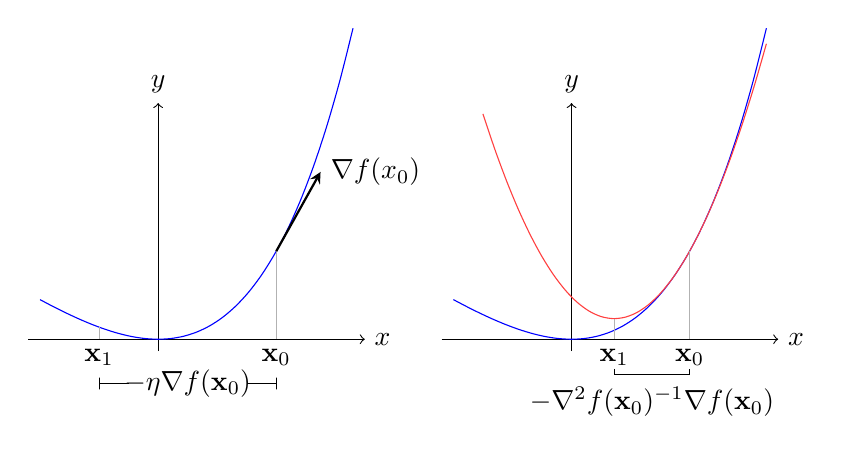
\begin{tikzpicture}[scale=0.75]
            \begin{scope}[shift={(-3.5,0)}]
                \draw[->] (-2.2,0) -- (3.5,0) node[right] {$x$};
                \draw[->] (0,-0.2) -- (0,4) node[above] {$y$};
                \draw[domain=-2:3.3,
                      smooth,
                      variable=\x,
                      blue] plot ({\x},{exp(\x/5)*\x*\x/4});
                \draw (2,0) node[below]{$\xx_0$};
                \draw[color=black!30] (2,0) -- (2,{exp(2/5)});
                \draw[thick,-stealth] (2,1.49) -- ++(0.75,{1.79*0.75}) node[right] {$\nabla f(x_0)$};
                \draw (-1,0) node[below]{$\xx_1$};
                \draw[color=black!30] (-1,0) -- (-1,{exp(-1/5)/4});
                \draw (-1,-0.75) -- ++(0,0.1) -- ++(0,-0.2) -- ++(0,0.1) -- ++(0.5,0);
                \draw (2,-0.75) -- ++(0,0.1) -- ++(0,-0.2) -- ++(0,0.1) -- ++(-0.5,0);
                \draw (0.5,-0.75) node {$-\eta\nabla f(\xx_0)$};
            \end{scope}
            \begin{scope}[shift={(3.5,0)}]
                \draw[->] (-2.2,0) -- (3.5,0) node[right] {$x$};
                \draw[->] (0,-0.2) -- (0,4) node[above] {$y$};
                \draw[domain=-2:3.3,
                      smooth,
                      variable=\x,
                      blue] plot ({\x},{exp(\x/5)*\x*\x/4});
                \draw[domain=-1.5:3.3,
                      smooth,
                      variable=\x,
                      red!75] plot ({\x},{1.49182 + 1.79019*(\x-2) + 0.701158*(\x-2)*(\x-2)});
                \draw (2,0) node[below] {$\xx_0$};
                \draw[color=black!30] (2,0) -- (2,1.49182);
                \draw (0.723404,0) node[below] {$\xx_1$};
                \draw[color=black!30] (0.723404,0) -- (0.723404,0.34915);
                \draw (0.723404,-0.5) -- ++(0,-0.1) -- ++({2-0.723404},0) -- ++(0,0.1);
                \draw ({(2+0.723404)/2},-0.65) node[below] {$-\nabla^2f(\xx_0)^{-1}\nabla f(\xx_0)$};
            \end{scope}
        \end{tikzpicture}
    \end{center}
\end{frame}

\begin{frame}
    \frametitle{Newton's Method}
    Approximating $f$ as a quadratic with it's Taylor Expansion:
    \[
        f_{\xx_0}(\xx) \approx f(\xx_0) + \nabla f(\xx_0)^\T (\xx - \xx_0) + \frac{1}{2}(\xx - \xx_0)^\T \nabla^2 f(\xx_0) (\xx - \xx_0).
    \]
    At optimality we have
    \[
        \nabla \widetilde f = \nabla f + \nabla^2 f (\xx - \xx_0) = 0,
    \]
    so
    \[
        \xx^\star = \xx_0 - \nabla^2 f^{-1} \nabla f.
    \]
\end{frame}

\begin{frame}
    \frametitle{Newton's Method}
    \begin{algorithm}[H]
        \SetKwInOut{Input}{input}\SetKwInOut{Output}{output}
        \textbf{Newton's Method}\\
        \Input{$f$, $\nabla f$, $\nabla^2f$, starting point $\xx_0$, tolerance $\epsilon$}
        \Output{optimal point $\xx^\star$}
        $t \leftarrow 0$\\
        \While{$|| \nabla f ||_2 \geq \epsilon$}{
            solve $\nabla^2 f(\xx_t) \dd_t = \nabla f(\xx_t)$ for $\dd_t$\\
            $\xx_{t+1} \leftarrow \xx_t - \dd_t$\\
            $t \leftarrow t + 1$
        }
        \textbf{return } $\xx^\star = \xx_{t+1}$
    \end{algorithm}
\end{frame}

\begin{frame}
    \frametitle{Newton's Method is Good}
    \begin{center}
        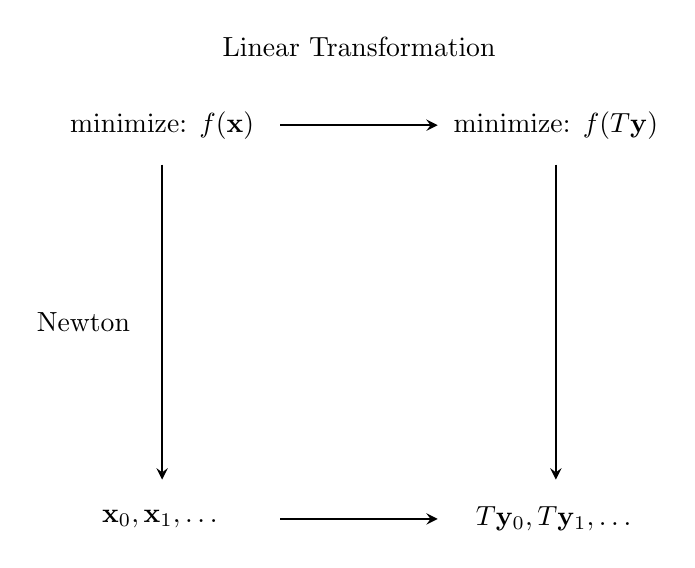
\begin{tikzpicture}
            \draw (0,5) node {minimize: $f(\xx)$};
            \draw (0,0) node {$\xx_0, \xx_1, \dots$};
            \draw (5,5) node {minimize: $f(T\yy)$};
            \draw (5,0) node {$T\yy_0, T\yy_1, \dots$};

            \draw[-stealth, thick] (1.5,5) -- (3.5,5);
            \draw[-stealth, thick] (0,4.5) -- (0,0.5);
            \draw[-stealth, thick] (1.5,0) -- (3.5,0);
            \draw[-stealth, thick] (5,4.5) -- (5,0.5);

            \draw (-1,2.5) node {Newton};
            \draw (2.5,6) node {Linear Transformation};
        \end{tikzpicture}
    \end{center}
\end{frame}


\begin{frame}
    \frametitle{Newton's Method is Scale Invariant}
    \begin{proof}
        (Induction) Assume $\xx_t = A\yy_t$.
        Recall at each step
        \[
            \xx_{t+1} = \xx_t - \nabla^2 f^{-1} \nabla f.
        \]
        If we have $g(\yy) = f(A\yy) = f(\xx)$, then as before we have
        \[
            \nabla g = A^T\nabla f(\xx) \qquad\text{and}\qquad \nabla^2 g = A^T \nabla^2 f(\xx) A

        \]
        and then
        \begin{align*}
            \yy_{t+1} &= A^{-1}\xx_t - (A^T \nabla^2 f(\xx_t) A)^{-1} A^T\nabla f(\xx_t)\\
            &= A^{-1}\xx_t - A^{-1} \nabla^2 f(\xx_t)^{-1} A^{-\T} A^T\nabla f(\xx_t)\\
            &= A^{-1}\left[\xx_t - \nabla^2 f(\xx_t)^{-1}\nabla f(\xx_t)\right]\\
            A\yy_{t+1} &= \xx_{t+1}.
        \end{align*}
    \end{proof}
\end{frame}

\section{Recap}

\end{document}
